%%% Моделирование %%%
\section{Моделирование}

Во время селективного спекания порошкового металла под воздействием лазеров или пучков электронов, энергия от них вызывает нагрев частиц порошка на поверхности. 
При этом в точке воздействия источника энергии образуется область, где образуется бассейн рассплавленного металла, который в последествии застывает и соединяется с предыдущими областями, создавая непрерывную деталь.

Моделирование поведения компоненнтов в этой области -- потери от испарения, диффузия, конвекция, плавление и застывание -- позволяет судить об итоговом составе получившейся детали и, как следствие, о её механических свойствах и микроструктуре.

\subsection{Нульмерная модель}

% Процесс селективного плавления -- очень сложный. В нём играют роль различные процессы -- конвекция Марангони, поверхностное натяжение, давление отдачи от испарения. 
В процессе движения по засыпанному слою порошка, область расплава следует за источником и через какое-то время её размеры перестают расти и до смены направления движения сохраняются около определённого значения. 
Поэтому в данной модели рассматривается поведение концентраций компонентов в предположении бесконечно быстрой диффузии в бассейне расплава неизменной 
прямоугольной формы. На рисунке \ref{fig:zero-model} изоражена геометрическая интерпретация модели.

Уравнение на потоки \ref{eq:zero-general} и формулы для каждого потока выглядят следующим образом \ref{eq:zero-melt} - \ref{eq:lambda}:
\begin{equation}
    \label{eq:zero-general}
    \dot{m} = j_{melt} - j_{solid} - j_{evap}
\end{equation}
\begin{equation}
    \label{eq:zero-melt}
    j_{melt} = \lambda m
\end{equation}
\begin{equation}
    \label{eq:zer-sol}
    j_{solid} = \lambda m_0
\end{equation}
\begin{equation}
    \label{eq:lambda}
    \lambda = \frac{v_{beam}}{L}
\end{equation}

\noindent
здесь $v_{beam}$ -- скорость сканирования, а $m$ и $m_0$ -- текущая и начальная масса содержимого бассейна.

Таким образом уравнения \ref{eq:zero-general} - \ref{eq:lambda} в связке с уравнениями для рассчёта испарения \ref{eq:evap} - \ref{eq:cc} формируют систему, описывающую данную нульмерную модель.

Стоит отметить, что данная модель не учитвает многокомпонентности, а уравнение \ref{eq:zero-general} может быть решено аналитически:

\begin{equation}
    m = m_0 -\frac{j^{evap}}{\lambda} (1 - e^{-\lambda t})
\end{equation}
\begin{equation}
    \lim_{t\rightarrow \infty } m = m_0 - \frac{j^{evap}}{\lambda}
\end{equation}

\addimg{zero-model-view.pdf}{0.8}{Нульмерная модель бассейна расплава. Здесь $j_{evap}$ -- поток испарения, $j_{melt}, j_{solid}$ -- потоки приходящего (плавящегося) и уходящего (застывающего) вещества соотвественно, определяемые скоростью движения источника.}{fig:zero-model}

На рис. \ref{fig:anal-solution} изображено решение для бассейна расплавленного алюминия температурой 3000К, диаметром источника 0.1 мм, размеры бассейна раплава -- 1000\times300\times100 мкм -- длина, ширина и глубина соответственно. Параметры матриала, необходимые для рассчёта испарения были взяты из работы \cite{klassen2018simulation}.

\addimg{anal_solution.pdf}{1.0}{Аналитическое решение уравнения \ref{eq:zero-general}}{fig:anal-solution}

Однако для уравнения, записанного двух компонент компонент  \ref{eq:zero-double-comp} аналитическое решение гораздо сложнее и в этой работе оно считается численно. 

\begin{equation}
    \label{eq:zero-double-comp}
    \dot{m_{\alpha}} = -j_{\alpha} \gamma^{\text{акт}}_{\alpha} \frac{\mu_{\alpha}}{m_{\alpha}}\frac{1}{\sum\limits_{\alpha} \frac{\mu_{\alpha}}{m_{\alpha}}} + \lambda (m_{\alpha}^0 - m_{\alpha})
\end{equation}

\addimg{thesis-w-3000.pdf}{1.0}{Численное решение уравнения \ref{eq:zero-general}}{fig:test}

\begin{figure}
    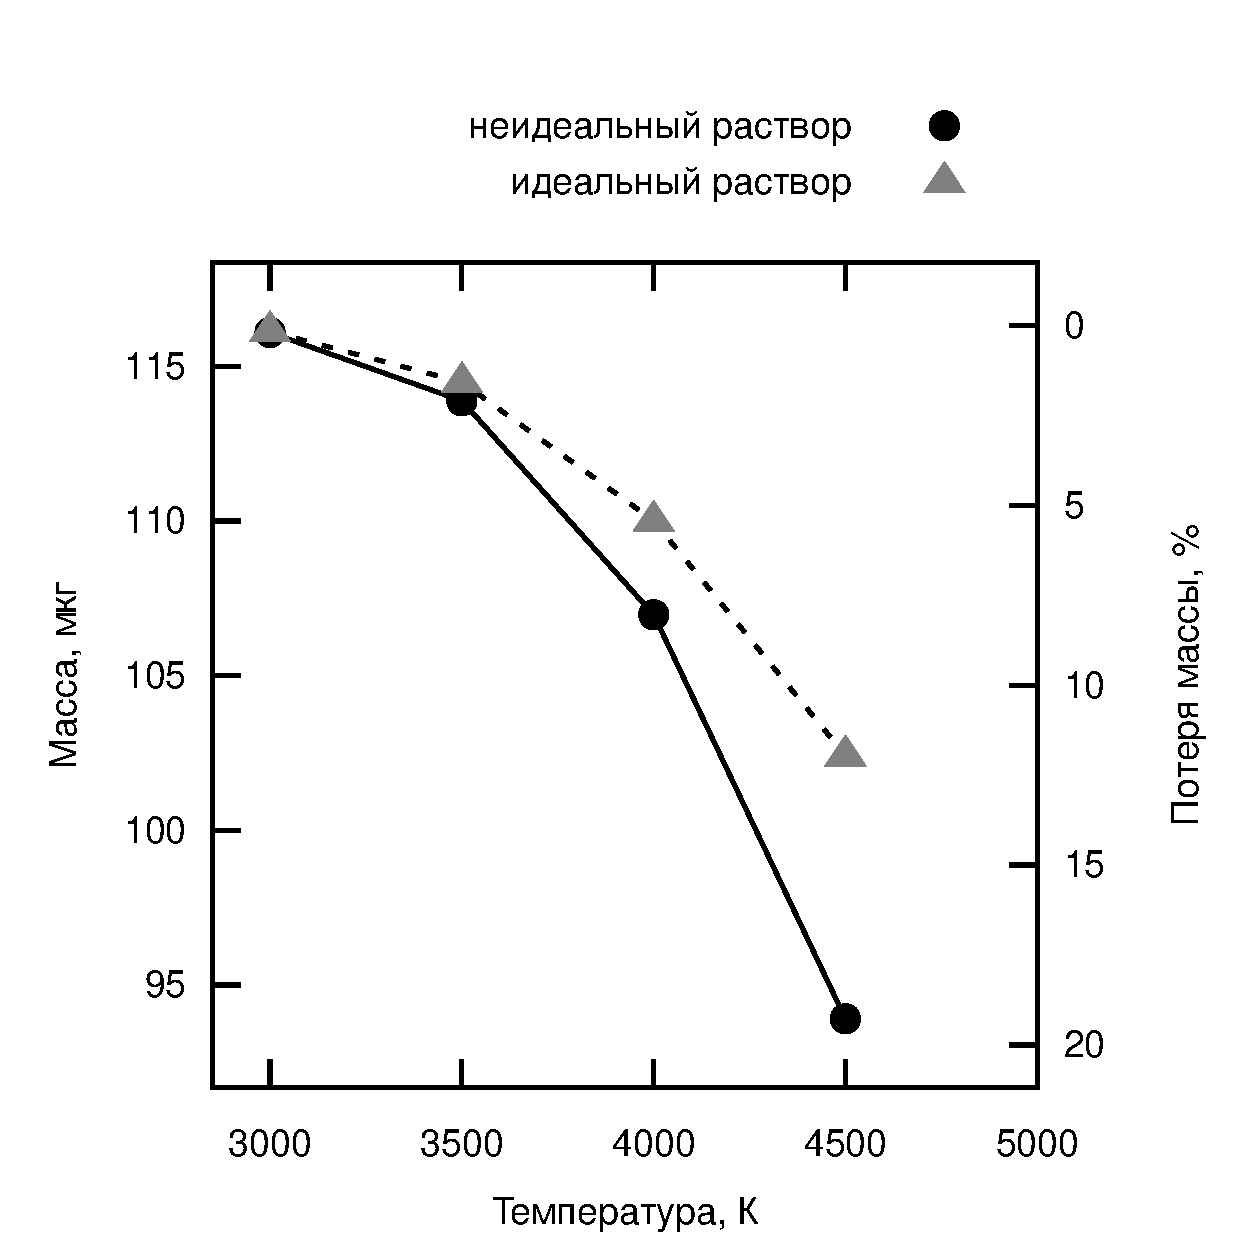
\includegraphics[width=.5\textwidth]{thesis-w-all.pdf}\hfill
    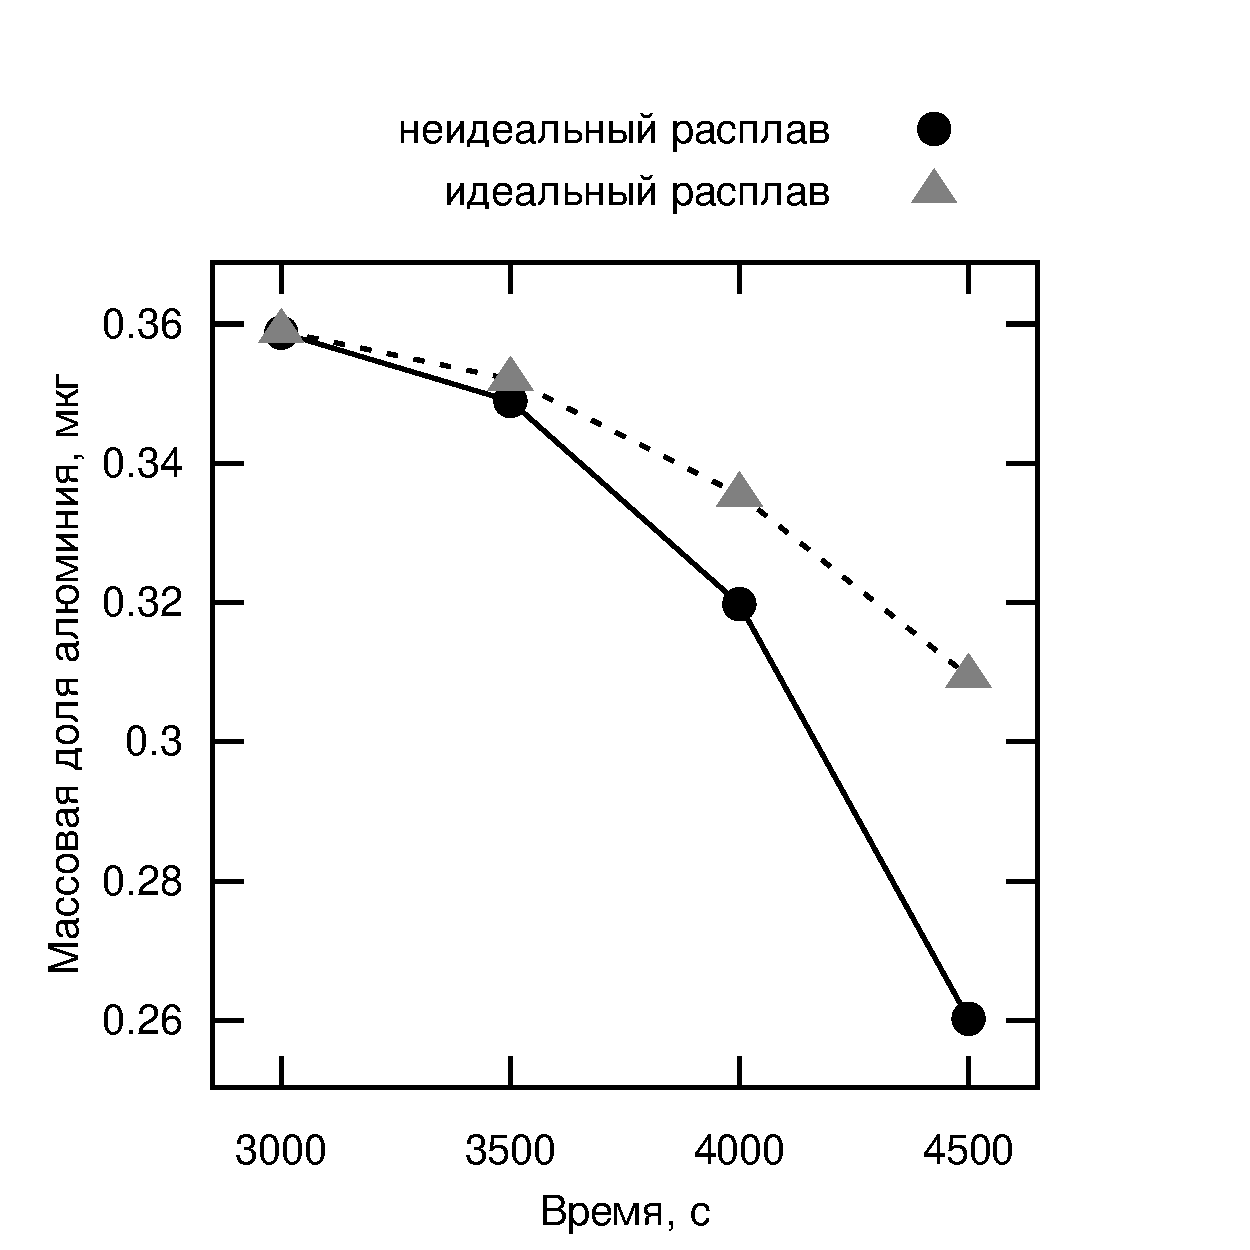
\includegraphics[width=.5\textwidth]{thesis-cwwo-all.pdf}\hfill
    \caption{Потери в сплаве TiAl по прошествии 0.01с при разынх температурах с учётом неидеальности и без. На рисунке слева общая потеря массы материала, на рисунке справа массовая доля алюминия.}
\end{figure}

\subsection{Трёхмерная модель}

Однако чтобы лучше описывать и исзучать динамику компонентов в этом процессе необходимо учитывать больше эффектов. К примеру диффузия и конвекция компонентов под поверхностью испарения может приводить к тому, что концентрация легколетучего компонента у поверхности сильно снижается и, следовательно, испаряться будет гораздо меньше.

Следующая модель описывает теплопроводность, теплоту плавления, конвекцию марангони и диффузию компонентов в расплаве.

На прямоугольной области -- подложке -- решается уравнение теплопроводности \ref{eq:heat}.

\begin{equation}
    \label{eq:heat}
    \frac{\partial h}{\partial t} = \alpha\left(\frac{\partial^2 T}{\partial x^2} + \frac{\partial^2 T}{\partial y^2} + \frac{\partial^2 T}{\partial z^2}\right),
\end{equation}
где $\alpha = \chi \rho^{-1} $, $h$ -- удельная энтальпия, $\chi$ -- коэффициент теплопроводности, $\rho$ -- плотность. Важно отметить, что в уравнении в левой части стоит энтальпия. Она связывается с температурой по формуле \ref{eq:enthal}, как уже было описано выше.

Граничное условие для этого уравнения представляют из себя постоянное значение $T_{amb} = 300K$ на всех границах, кроме верхней, контактирующей с атмосферой и через которую идёт испарение. На этой границе устанавливается граничное условие на поток. В него входит как источник $q_{source}$, так и потери $q_{evap}$ -- уравнение \ref{eq:bound_cond_heat}.

\begin{equation}
    \label{eq:bound_cond_heat}
    \chi \frac{\partial T_{\Gamma}}{\partial z}  \big|_{z=0} = q_{source} - q_{evap},
\end{equation}

Однако в жизни всё сложнее и очень сильное влияние на теплоперенос оказывает конвекция, связанная с гидродинамикой и которая в данной работе напрямую не моделируется. Но конвекцию, связанную с эффектом Марангони возможно описать эффективным коэффицентом теплопроводности, как это показано в \ref{eq:keff} выше. 

Следующий важный шаг в построении модели это описать поведение компонентов расплава в самом бассейне. Особенно важно это сделать потому, что от того, как металлы себя поведут и в каких концентрациях они окажутся у поверхности, будет зависеть то, сколько какого компонента в итоге испарится. В этой модели описывается перенос за счёт диффузии. В области расплава решается уравнение \ref{eq:diffusion}.

\begin{equation}
    \label{eq:diffusion}
    \frac{\partial c}{\partial t} = D\left(\frac{\partial^2 c}{\partial x^2} + \frac{\partial^2 c}{\partial y^2} + \frac{\partial^2 c}{\partial z^2}\right)
\end{equation}

Граничные условия для этого уравнения задаются следующим образом. На границе с твёрдой фазой поток задаётся равным нулю \ref{eq:diff_solidbc}, а на границе с газом \ref{eq:diff_gasbc} -- поток испарения. Если температуры для испарения будет недостаточно, то поток испарения будет просто равен нулю.

\begin{equation}
    \label{eq:diff_solidbc}
    D \frac{\partial c}{\partial x} = 0.
\end{equation}

\begin{equation}
    \label{eq:diff_gasbc}
    D \frac{\partial c}{\partial z} = -j_{evap}(T)
\end{equation}

\subsection{Численная схема}

Описанная в этой работе трёхмерная модель реализовывалась для расчёта на графических процессорах. Это несёт целый ряд преимуществ: высокая производительность в решении задач, которые можно разбить на большое количество задач более мелких, а так же возможность легко масштабировать программу для более мощных ресурсов.

Чтобы использовать преимущества графического процессора, было решено использовать явную схему для решения уравнений теплопроводности и диффузии:

\begin{multline}
    \label{eq:heat_scheme}
    \frac{h^{k+1}_{n,m,l} - h^{k}_{n,m,l}}{\Delta t} = \alpha \bigl( \frac{T^k_{n-1, m,l} - 2T^k_{n,m,l} + T^k_{n+1,m,l}}{h_x^2} + \\
    + \frac{T^k_{n, m-1,l} - 2T^k_{n,m,l} + T^k_{n,m+1,l}}{h_y^2} + \frac{T^k_{n, m,l-1} - 2T^k_{n,m,l} + T^k_{n,m,l+1}}{h_z^2} \bigr)
\end{multline}

\begin{multline}
    \label{eq:diff_scheme}
    \frac{c^{k+1}_{n,m,l} - c^{k}_{n,m,l}}{\Delta t} = D\bigl( \frac{c^k_{n-1, m,l} - 2c^k_{n,m,l} + c^k_{n+1,m,l}}{h_x^2} + \\
     + \frac{c^k_{n, m-1,l} - 2c^k_{n,m,l} + c^k_{n,m+1,l}}{h_z^2} + \frac{c^k_{n,m,l-1} - 2c^k_{n,m,l} + c^k_{n,m,l+1}}{h_x^2}\bigr)
\end{multline}

\noindent 
Здесь индекс $k$ означает шаг по времени, индексы $n, m, l$ -- по координатам $x, y, z$ соответственно. 

Граничные условия для уравнения теплопроводности из \ref{eq:bound_cond_heat} становятся \ref{eq:bound_cond_heat_scheme}.

\begin{equation}
    \label{eq:bound_cond_heat_scheme}
    \chi \frac{T^k_{n,m,l} - T^k_{n,m,l-1}}{\Delta z}  \big|_{z=0} = q_{source} - q_{evap},
\end{equation}

Чтобы понять как устроены граничные условия для уравнения диффузии можно посмотреть на рисунок \ref{fig:diff_bound_cond}. На нём изображено возможное окружение ячейки с жидкостью. Сверху газ, с которым граничное условие -- поток $j_{evap}$. Справа и снизу -- твёрдая фаза, 
следовательно поток равен нулю. Наконец, граница на границе с жидкостью уравнение считается как обычно.

\addimg{diff_bound_cond.pdf}{0.9}{Наглядно продемонстрированные граничные условия на уравнение диффузии.}{fig:diff_bound_cond}

\sunsection{Валидация модели}



\subsection{Модель конвекции}

\begin{equation}
    \label{eq:sec-upwind}
    \frac{c^{n+1}_{i} - c^{n}_{i}}{\Delta t} =
    \begin{cases}
         -\frac{v_i}{2\Delta x_i}(3u_i-4u_{i-1}+u_{i-2}), &v_i > 0 \\
         \frac{v_i}{2\Delta x_i}(3u_i-4u_{i+1}+u_{i+2}), &v_i < 0 
    \end{cases}
\end{equation}

\clearpage